\documentclass[10pt]{article}
\usepackage[margin=0.9in]{geometry}
\usepackage{amsmath,amssymb}
\usepackage{graphicx}
\usepackage{booktabs}
\usepackage{tabularx}
\usepackage{xcolor}
\usepackage[hidelinks]{hyperref}
\usepackage{titlesec}
\usepackage{enumitem}
\definecolor{indigo}{HTML}{1C2757}
\titleformat{\section}{\large\bfseries\color{indigo}}{\thesection}{0.6em}{}
\titleformat{\subsection}{\normalsize\bfseries\color{indigo}}{\thesubsection}{0.6em}{}
\setlength{\parindent}{0pt}
\setlength{\parskip}{4pt}
\setlist{itemsep=1pt,topsep=2pt}
\newcommand{\pd}[2]{\frac{\partial #1}{\partial #2}}

\begin{document}

{\color{indigo}\small\bfseries EQUIPHYSICS · HORSE ARTERY LAB}\\[2pt]
{\color{indigo}\LARGE\bfseries The horse artery model: equations and parameters}\\[4pt]
{\itshape A Python version of Vera et al.\ (2019), \emph{PLoS ONE} 14(8): e0221425. EquiPhysics, October 2026.}

\section{What the model is}
The model follows blood pressure $P(x,t)$ and flow $Q(x,t)$ along 117 arteries of a resting warmblood horse, from
the aortic root to the head, the four legs, and the abdominal organs (Fig.~\ref{fig:tree}). A time-varying
elastance left ventricle drives the tree; 62 three-element Windkessels close it. Anatomy (length, branching angle,
tapered lumen diameter, and distensibility of each segment) is the study's Table~1; terminal resistances and
compliances are its S1 Table. Both are open access under CC~BY~4.0. The study's MATLAB code is not public; our choices
where the article is silent are marked \emph{ours} below.

\begin{figure}[h]
\centering
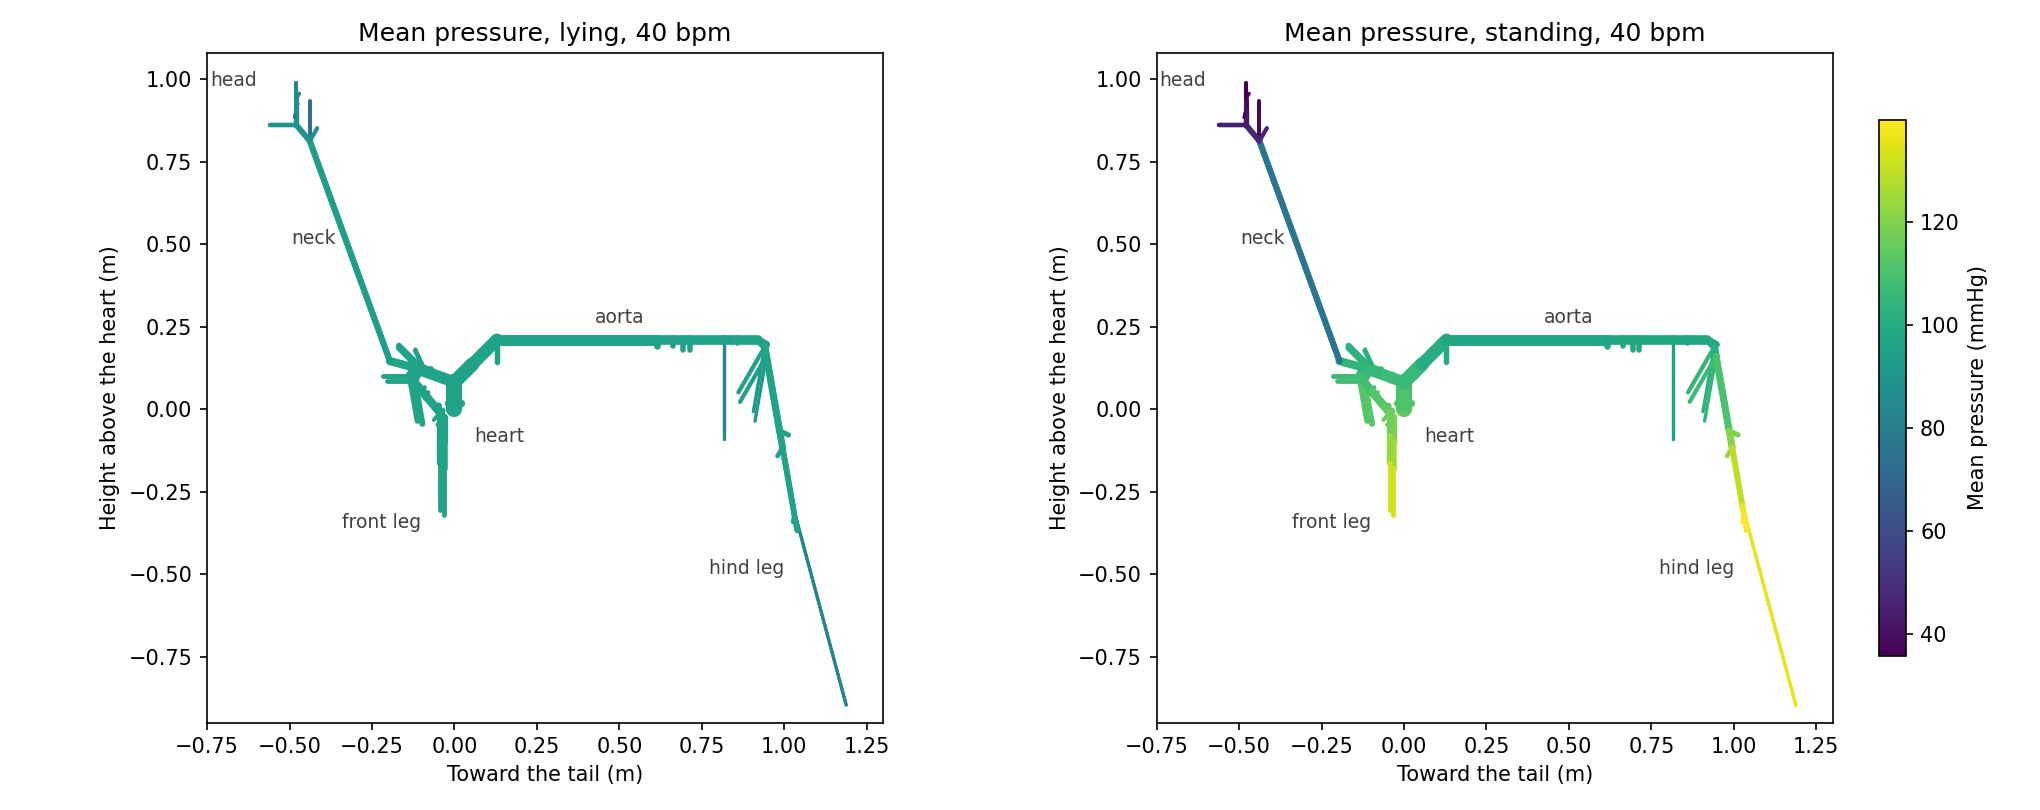
\includegraphics[width=\textwidth]{../figures/fig_map_mean_lying_standing.png}
\caption{The 117 segments drawn from their lengths and angles (horse facing left), colored by mean pressure in a
resting horse lying (left) and standing (right), on one color scale.}
\label{fig:tree}
\end{figure}

\section{Equations in each artery}
With $x$ along the segment, $A$ the lumen area, $R=\sqrt{A/\pi}$, and $\rho$, $\mu$ the blood density and viscosity,
\begin{align}
C_A(x,P)\,\pd{P}{t} + \pd{Q}{x} &= 0, \label{eq:mass}\\
\pd{Q}{t} + \pd{}{x}\!\left(\delta\,\frac{Q^2}{A}\right) + \frac{A}{\rho}\pd{P}{x} &= \frac{2\pi R}{\rho}\,\tau_w - A\,g\sin\varphi . \label{eq:mom}
\end{align}
Equation~\eqref{eq:mass} is conservation of mass ($\partial A/\partial t + \partial Q/\partial x = 0$ with $A=A(x,P)$);
\eqref{eq:mom} is the cross-section-averaged momentum balance. $\varphi$ is the segment's angle in the side view
(0$^\circ$ toward the tail, 90$^\circ$ up), so the last term is gravity along the vessel. $\delta$ is the
momentum-flux coefficient: 1 (flat profile) where the Womersley number exceeds 3, $4/3$ (Poiseuille) elsewhere (\emph{ours}).

\paragraph{Wall law.} The area compliance follows the study's Eq.~(3): a reference distensibility $D$ (Table~1, per
segment) times a pressure-dependent factor,
\begin{equation}
C_A(x,P) = A_{\mathrm{ref}}(x)\,D\,\frac{C_p(P)}{C_p(P_{\mathrm{ref}})},\qquad
C_p(P) = a_1 + \frac{b_1}{1+\big((P-P_{\max C})/P_{\mathrm{width}}\big)^2}.
\end{equation}
Integrating gives the area, with $F(P) = a_1P + b_1P_{\mathrm{width}}\arctan\!\big((P-P_{\max C})/P_{\mathrm{width}}\big)$:
\begin{equation}
A(x,P) = A_{\mathrm{ref}}(x)\left[1 + D\,\frac{F(P)-F(P_{\mathrm{ref}})}{C_p(P_{\mathrm{ref}})}\right].
\end{equation}
$A_{\mathrm{ref}}(x)$ tapers linearly in radius between the proximal and distal diameters of Table~1. The wall stiffens as
pressure rises, so the wave speed $c=\sqrt{A/(\rho C_A)}$ grows with pressure. The characteristic impedance is $Z=\rho c/A$.
Below a quarter of the reference area we continue the law with a smooth exponential collapse (\emph{ours}); normal runs
never reach it.

\paragraph{Wall friction (Witzig--Womersley).} Where $\alpha=R\sqrt{\omega\rho/\mu}>3$ at the heart rate $\omega$, the
wall shear stress comes from the harmonics $Q_n$ of the flow (study's Eq.~6):
\begin{equation}
\tau_w(t) = -\frac{4\mu}{\pi R^3}\,\bar Q + \sum_{n=1}^{N}\mathrm{Re}\!\left\{\frac{\mu}{\pi R^3}\,
\mathcal F(\Lambda_n)\,Q_n\,e^{in\omega t}\right\},\quad
\mathcal F(\Lambda)=\frac{\Lambda\,J_1(\Lambda)/J_0(\Lambda)}{1-2J_1(\Lambda)/\big(\Lambda J_0(\Lambda)\big)},\quad
\Lambda_n=\alpha\sqrt{n}\,i^{3/2}.
\end{equation}
$\mathcal F\to-4$ (Poiseuille) as $\alpha\to0$ and $|\mathcal F|\sim\alpha$ for large $\alpha$. As in the study, the
harmonics come from the previous beat; we add a Poiseuille correction for the change in flow since then, which
vanishes once the solution is periodic (\emph{ours}). $N=30$ (\emph{ours}). Elsewhere $\tau_w=-4\mu Q/(\pi R^3)$.

\section{Boundary conditions}
\paragraph{Heart.} A time-varying elastance with an internal resistance (study's Eqs.~10--11):
\begin{equation}
P_{\mathrm{LV}} = E^*(t)\,\big[1-\kappa Q(t)\big]\,(V-V_0),\qquad
E^*(t) = E_{\min} + (E_{\max}-E_{\min})\,e(t),
\end{equation}
where $e(t)$ is a normalized double-Hill curve (Stergiopulos et al.\ 1996, fit to Senzaki et al.\ 1996) peaking at
$T_{\max}$ (\emph{ours}). The aortic valve is open while $Q>0$, and then $P_{\mathrm{LV}}$ equals the root pressure. When
$P_{\mathrm{LV}}$ falls below the filling pressure the ventricle fills at $(P_{\mathrm{fill}}-P_{\mathrm{LV}})/R_{\mathrm{fill}}$.

\paragraph{Branch points.} Pressure is continuous and flow is conserved: $P$ is the same in the parent and all
daughters, and $Q_{\mathrm{parent}}=\sum Q_{\mathrm{daughters}}$. The equine tree has two-, three-, and four-way branchings
(the carotid ends in three branches; the aorta ends in a quadrifurcation).

\paragraph{Terminal beds.} A 3-element Windkessel (study's Eq.~7) at each of the 62 ends:
\begin{equation}
P = P_c + R_1 Q,\qquad C_T\,\frac{dP_c}{dt} = Q - \frac{P_c-P_{\mathrm{out}}}{R_2},
\end{equation}
with total resistance $R_T=R_1+R_2$ and compliance $C_T$ from the S1 Table and $R_1=Z_c$ (no reflection at high
frequency). In nine small head branches $Z_c>R_T$; there $R_1=R_T$, $R_2=0$ (\emph{ours}). $P_{\mathrm{out}}=0$.

\section{Numerical method (ours)}
The study used an implicit finite-difference scheme. We use an explicit MacCormack scheme in the interior (sweep
direction alternating each step) and the method of characteristics at every segment end: along $dx/dt=u\pm c$ the
quantities $W_\pm = P\pm ZQ$ (plus the source term) carry information to the boundary, where they are combined with
the heart, branch, or Windkessel conditions. A Jameson-type shock-capturing damping keeps the steepening pulse front
from ringing. Grid spacing 10~mm (1{,}111 points), time step about 0.16~ms (CFL 0.8). Runs start from 100~mmHg and
1~ml/s (as in the study) and repeat beat to beat after about seven beats; we report the last beat of eight (the
notebook) or ten (the comparison script), which agree to the digits shown. Halving the grid spacing changes the
reported numbers by 1--2\%.

\section{Parameters}
\begin{center}
\small
\begin{tabularx}{\textwidth}{@{}lXll@{}}
\toprule
Group & Parameter & Value & Source \\
\midrule
Blood & density $\rho$; viscosity $\mu$ & 1050 kg/m$^3$; 0.004 Pa\,s & study \\
Gravity & $g$; segment angles $\varphi$ & 9.81 m/s$^2$; Table 1 & study \\
Wall & $a_1$, $b_1$, $P_{\max C}$, $P_{\mathrm{width}}$, $P_{\mathrm{ref}}$ & 0.76, 5, 10 mmHg, 21 mmHg, 100 mmHg & study \\
 & distensibility $D$; diameters; lengths & per segment, Table 1 & study \\
Heart & heart rate; $T_{\max}$ & 40 beats/min; 478 ms & study (systolic duration) \\
 & $E_{\max}$; $E_{\min}$ & 0.26; 0.0127 mmHg/ml & study; calibrated (study: 0.01) \\
 & $\kappa$; $V_0$ & $55\times10^{-6}$ s/ml; 0 ml & study \\
 & filling pressure; filling resistance & 16 mmHg; 0.003 mmHg\,s/ml & study \\
 & elastance curve shape & double Hill: 0.303, 0.508, 1.32, 21.9 & ours (Stergiopulos 1996) \\
Terminals & $R_T$, $C_T$ & per terminal, S1 Table & study \\
 & $R_1$; $P_{\mathrm{out}}$ & $Z_c$ (or $R_T$ if smaller); 0 & study; ours \\
Friction & Womersley where $\alpha>3$; harmonics & --; 30 & study; ours \\
Numerics & $\Delta x$; CFL; damping $\kappa_2$; beats & 10 mm; 0.8; 1; 8--10 & ours \\
\bottomrule
\end{tabularx}
\end{center}
With every parameter as printed, the model pumps 39.6 L/min instead of the study's 33. The study's stroke volume
(820 ml) and ejection fraction (65\%) imply an end-diastolic volume near 1{,}260 ml, while $E_{\min}=0.01$ lets ours
fill to 1{,}530 ml. Matching that one number ($E_{\min}=0.0127$) is our only calibration; gravity is never tuned.

\section{How it compares with the study}
\begin{center}
\small
\begin{tabular}{@{}lcccc@{}}
\toprule
 & Study, lying & Ours, lying & Study, standing & Ours, standing \\
\midrule
Cardiac output (L/min) & 33 & 32.5 & 30 & 29.6 \\
Stroke volume (ml) & 820 & 812 & 740 & 740 \\
Aortic root pressure (mmHg) & 114/70 & 114/72 & 131/88 & 131/90 \\
Pulse pressure (mmHg) & 44 & 42 & 43 & 41 \\
Total vascular resistance (mmHg\,s/ml) & 0.17 & 0.18 & 0.22 & 0.23 \\
Aortic pulse wave speed (m/s) & 5.3 & 5.1 & 5.2 & 5.1 \\
\bottomrule
\end{tabular}
\end{center}
Mean flows (Reynolds numbers) at the five sites agree within 10\%, Womersley numbers within 6\%, and the waveform
shapes and the shift of blood from head to legs on standing match the study's figures. Peak velocities differ by up to
30\% at some sites, limb pulse pressures are 10--20\% lower than the study's, and peak wall shear depends on how many
harmonics are kept (the study does not say). Like the study's model, ours overestimates pulse pressure by about
70\%: 56 vs 33~mmHg in the carotid of standing horses, and 41 vs 24~mmHg at the aortic root (measured in one
anesthetized horse). Full tables: \texttt{results/comparison.md}.

\section{Teaching controls}
The notebook exposes three settings: \emph{standing} (gravity on or off), \emph{heart rate} (35--80 beats/min, with
$T_{\max}$ scaled by $\sqrt{40/\mathrm{HR}}$, ours), and \emph{stiffness} $s$ (every distensibility divided by $s$,
0.7--1.5). The model has no reflexes or autoregulation, so these show mechanics only. In a standing horse with a slow
heart and stiff arteries, head pressure can fall near zero before the next beat; the head arteries soften until blood
outruns the pressure wave and the 1D equations fail. The notebook reports this in plain words.

\section*{References}
\small
Vera L, Campos Arias D, Muylle S, Stergiopulos N, Segers P, van Loon G (2019). A 1D computer model of the arterial
circulation in horses: an important resource for studying global interactions between heart and vessels under
normal and pathological conditions. \emph{PLoS ONE} 14(8): e0221425.\\
Reymond P, Merenda F, Perren F, R\"ufenacht D, Stergiopulos N (2009). Validation of a one-dimensional model of the
systemic arterial tree. \emph{Am J Physiol Heart Circ Physiol} 297: H208--H222.\\
Stergiopulos N, Meister JJ, Westerhof N (1996). Determinants of stroke volume and systolic and diastolic aortic
pressure. \emph{Am J Physiol} 270: H2050--H2059.\\
Senzaki H, Chen CH, Kass DA (1996). Single-beat estimation of end-systolic pressure-volume relation in humans.
\emph{Circulation} 94: 2497--2506.\\
Womersley JR (1955). Method for the calculation of velocity, rate of flow and viscous drag in arteries when the
pressure gradient is known. \emph{J Physiol} 127: 553--563.\\
MacCormack RW (1969). The effect of viscosity in hypervelocity impact cratering. AIAA Paper 69-354.
\end{document}
